% Introduction Section

\section{Introduction}

\begin{frame}{Problem Statement}
\begin{itemize}
    \item \highlight{Legal document analysis} is crucial for contract review and compliance
    \item Traditional manual review is \highlight{time-consuming and error-prone}
    \item NLP models provide automation but lack \highlight{interpretability}
    \item Legal professionals need to understand \highlight{why} AI makes decisions
\end{itemize}

\vspace{0.5cm}
\begin{alertblock}{Research Question}
How can we develop explainable AI methods for automated legal clause extraction that provide interpretable insights for legal professionals?
\end{alertblock}
\end{frame}

\begin{frame}{Motivation}
\begin{columns}
\begin{column}{0.6\textwidth}
\textbf{Why Explainable AI in Legal Domain?}
\begin{itemize}
    \item \highlight{Regulatory compliance} requirements
    \item \highlight{Trust and transparency} for legal professionals
    \item \highlight{Error detection} and model debugging
    \item \highlight{Knowledge discovery} from legal patterns
\end{itemize}
\end{column}
\begin{column}{0.4\textwidth}
\begin{center}
% Show system architecture instead of placeholder
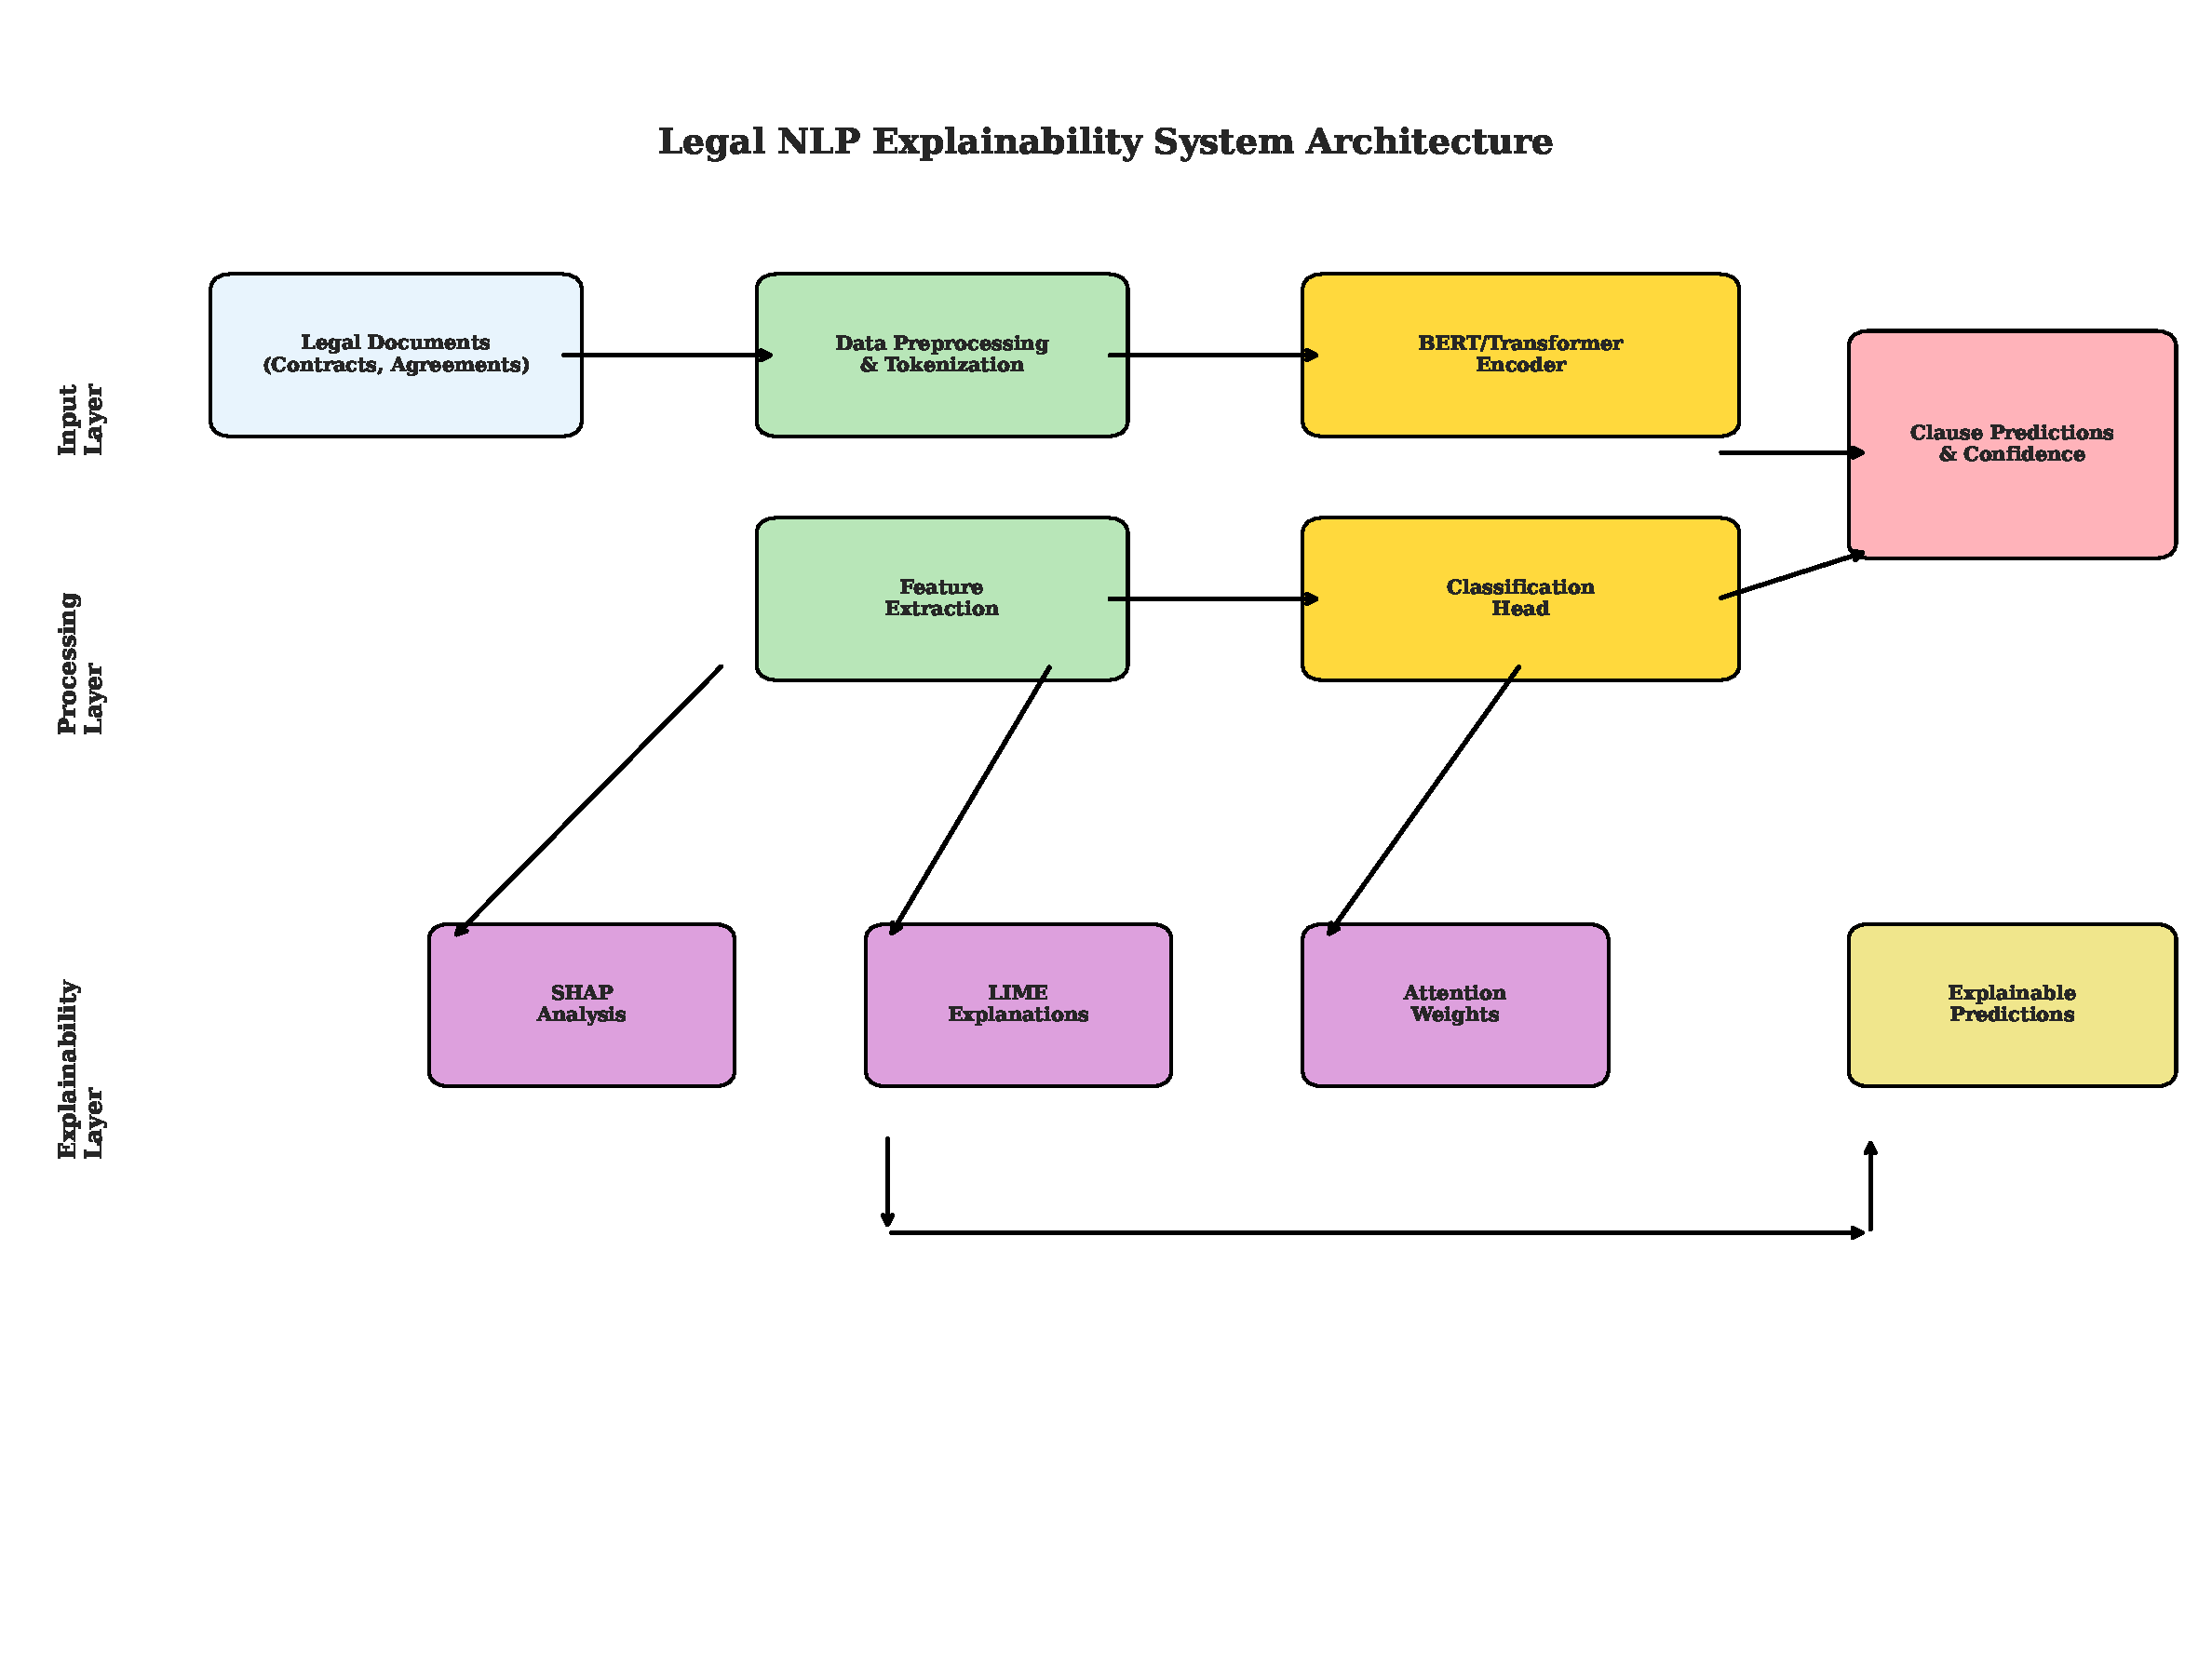
\includegraphics[width=\textwidth]{\figpath/system_architecture.pdf}
\end{center}
\end{column}
\end{columns}
\end{frame}

\begin{frame}{Project Scope}
\textbf{Objectives:}
\begin{enumerate}
    \item Develop a \highlight{BERT-based model} for clause extraction
    \item Implement \highlight{multiple explainability methods} (SHAP, LIME, Attention)
    \item Compare and evaluate \highlight{explanation quality}
    \item Create \highlight{interpretable visualizations} for legal professionals
\end{enumerate}

\vspace{0.5cm}
\textbf{Target Clauses:}
\begin{itemize}
    \item Termination clauses
    \item Limitation of liability
    \item Governing law
    \item Confidentiality provisions
    \item Payment terms
\end{itemize}
\end{frame}
